

\section{The Telegraph Process}\label{chapter:telegraph}

\textit{In this section we will develop a novel path-space framework for discrete-space, continuous-time Markov chains through consideration of the simplest such process, namely the telegraph process. We then validate our methods by recovering the time evolution and transient entropy production of the telegraph process through this new framework.}

\subsection{Known Results}
\begin{wrapfigure}{R}{0.4\textwidth}
\centering
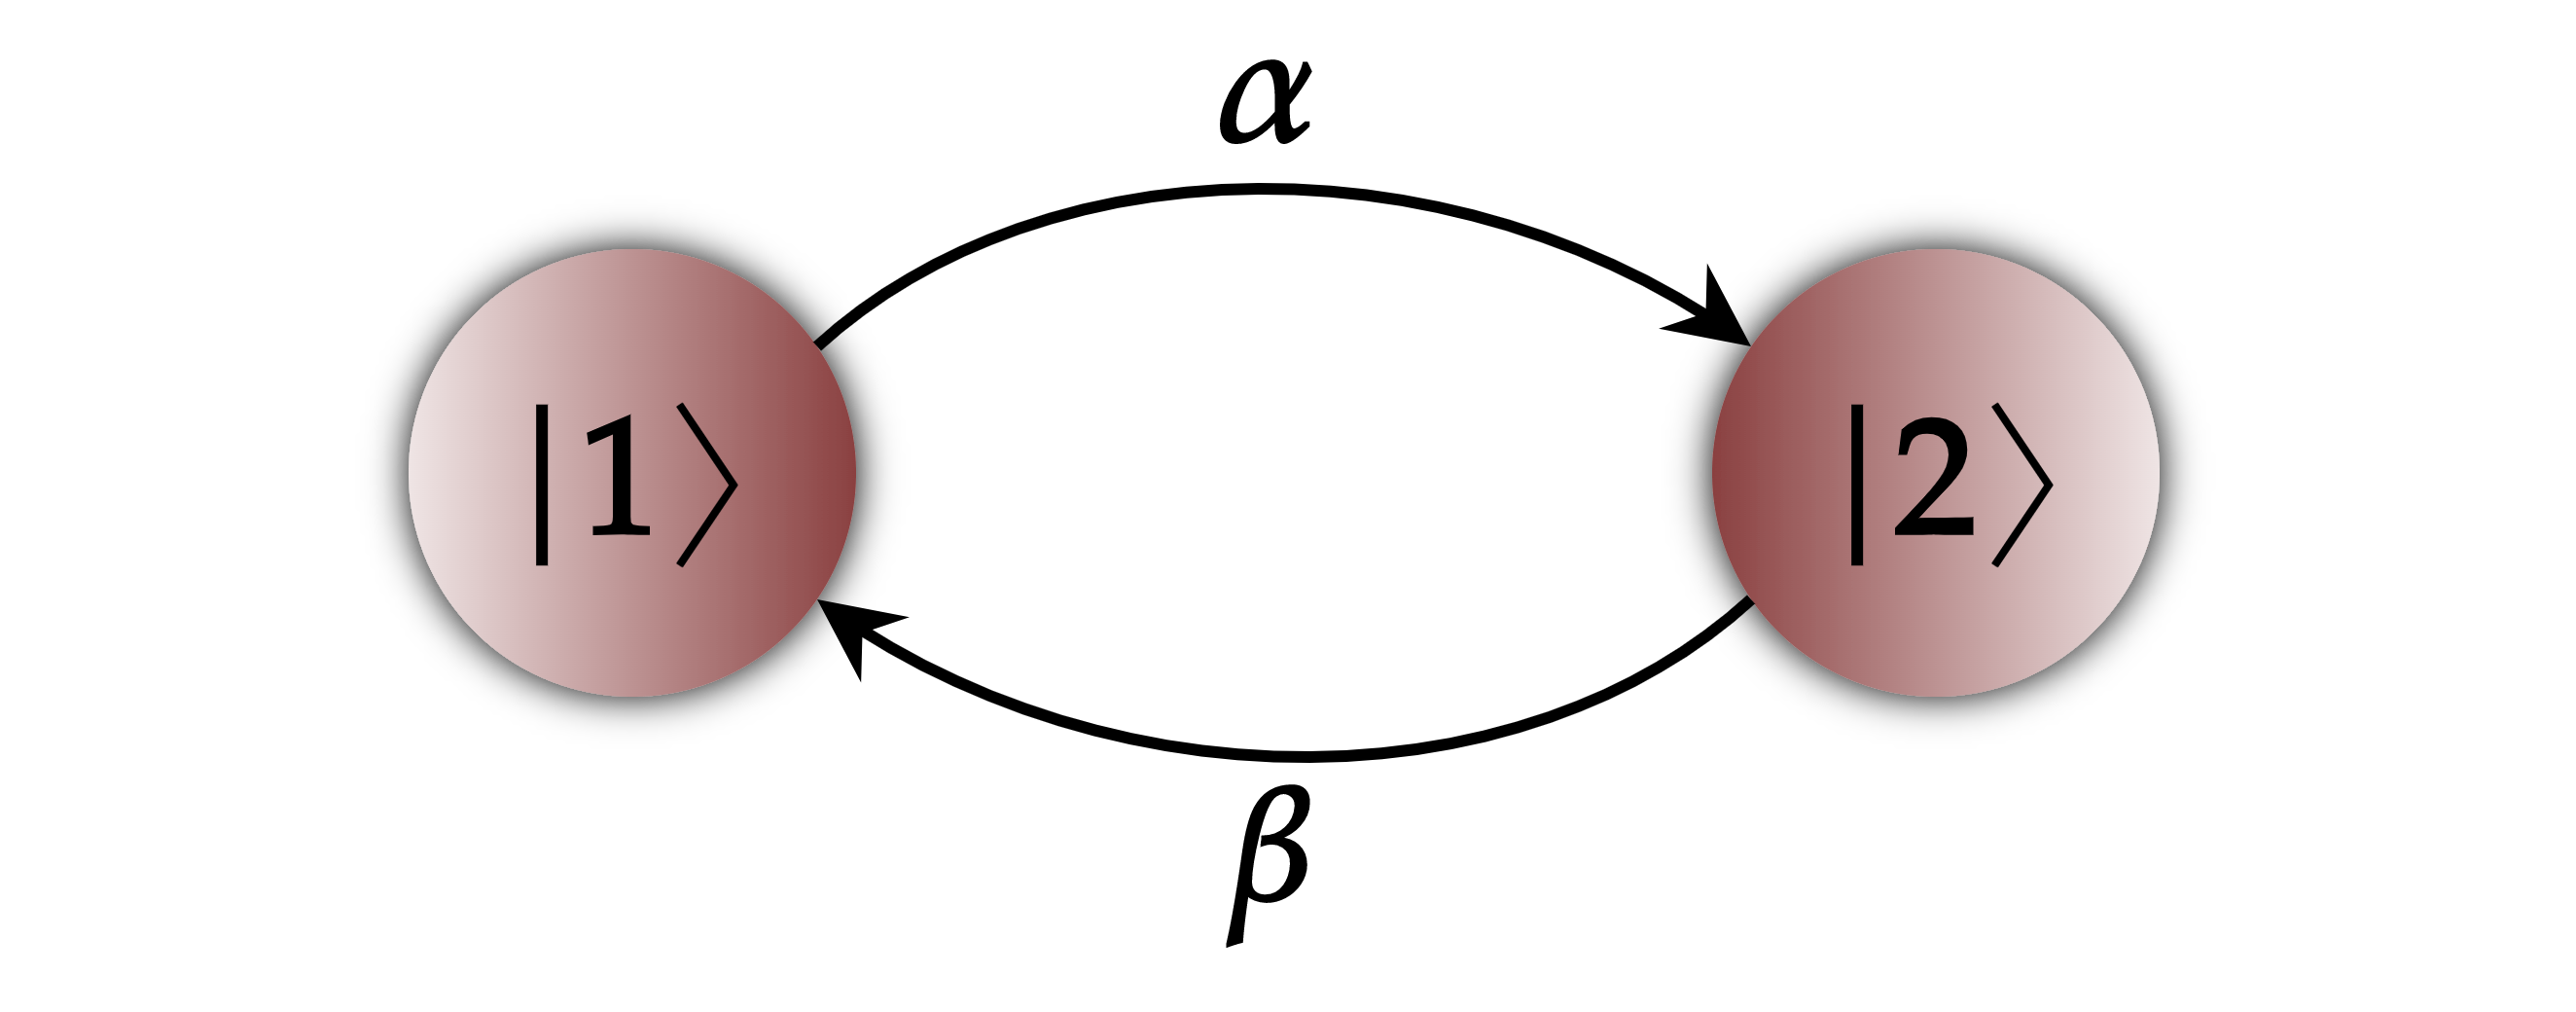
\includegraphics[width = 0.35\textwidth]{figures/tele-diagram-3.png}
\caption{\footnotesize Diagram of the telegraph process as described by Eqn. (\ref{two_state_transition_mat}). Regardless of the choice of initial condition, this system will settle into the equilibrium distribution $P(t) = \frac{1}{\alpha +\beta}(\beta\ket{1} + \alpha \ket{2})$. In this distribution the detailed balance conditions is satisfied, hence $\entpp = 0$ in the long-time limit.} 
\label{telegraph-diagram}
\end{wrapfigure}

The telegraph process is the continuous-time, two-state Markov chain described by the master equation

\begin{align}\label{two_state_transition_mat}
  \dot{P}(t) = P(t)e^{tW}, \; \; \; W = \begin{pmatrix}-\alpha && \alpha \\ \beta && -\beta \end{pmatrix}.
\end{align}


The telegraph process is a building block of more complicated processes which we will consider later in this text. For this reason, it is helpful to review some known results about its entropy production rate. Although the entropy production of discrete state-space Markov chains is usually considered from the stand point of graph theory, here we will replicate these results using a path-space formulation of entropy production. In this way we will develop some useful results by considering this simple system. This simple system will also provide a first stress test for our original framework for the derivation of path probabilities that we plan to use throughout much of this thesis. 

We will label the two states $\ket{1} $ and $\ket{2}$. We shall use the terms `particle' and `system' interchangeably, i.e. we may speak of the system or the particle being in state $\ket{1}$ etc. Given an initial condition $P(0) = P_0 = p\ket{1}  + (1-p)\ket{2} $, the system will evolve according to $P(t) = e^{tW}P_0$, and it will eventually reach the equilibrium distribution $P_\infty$, which is the normalised eigenvector of $e^{tW}$ with eigenvalue equal to one. Indeed

\begin{equation}\label{telegraph-state-prob}
  P(t) = A(t)\ket{1}  + B(t)\ket{2}  = \frac{1}{\alpha + \beta} \left((\beta + re^{-(\alpha + \beta)t})\ket{1}  +
(\alpha - re^{-(\alpha + \beta)t})\ket{2}  \right) ,
\end{equation}

with $r = \alpha p - \beta(1-p)$. The entropy productions rate of the telegraph process is then given by  \cite{cocconi2020entropy}

\begin{align}\label{telegraph-entropy-Luca}
  \entpp(t) &= re^{-(\alpha + \beta)t}\log \left(\frac{1+\frac{r}{\beta}e^{-(\alpha + \beta)t}}{1-\frac{r}{\alpha}e^{-(\alpha + \beta)t}}\right).
\end{align}


 The most immediate observation from this result is that the entropy production rate of the telegraph process converges exponentially to zero. This is consistent with the fact that at its stationary state the telegraph process obeys the detailed balance condition, so it does not allow any current. Markov processes with null current cannot produce any entropy. The exponential decay of the entropy production rate also reflects the exponential decay of the initial state to statistical equilibrium. Note the non-negativity of $\entpp$ for all choices of $\alpha$,$\beta$, and $t$. 

 In the following section we will recover (\ref{telegraph-state-prob}) and (\ref{telegraph-entropy-Luca}) through a novel path-space formulation. While recovering these results through a path-space formulation proves much more difficult than their original derivation through a state-space description, the path-space formulation will eventually allow us to deal with coarse-grained non-Markov systems that are not responsive to classical treatments.

\subsection{Path Probabilities}\label{two_state_path_prob}

Consider the discrete time, two-state Markov chain that evolves according to the matrix

\begin{equation}
M = \mathds{1} + \frac{t}{N}W, \; \; N \in \mathds{N},
\end{equation}

with $W$ as in (\ref{two_state_transition_mat}). This is the discretised analogue of the process described by (\ref{two_state_transition_mat}). The choice of $M$ as the stochastic matrix for this process is motivated by Proposition \ref{limit-of-mat} which states that\footnote{See Appendix A for an amusing proof of this proposition.}

\begin{align}
\lim_{N\rightarrow \infty}M^N = e^{tW}.
\end{align}

In the language of stochastic processes, $W$ is the generator of the Markov chain described by $M$. 

We prepare the system in $\ket{1}$, i.e. $p=1$. Then, given that the system starts in state $\ket{1} $, the probability of finding it there again after time $t/N$, having made no jumps, is given by $\bra{1} M\ket{1}  $. Moreover, the probability of the system making no jumps in time $t = Nt/N$ is

\begin{equation}
  \underbrace{\bra{1} M\ket{1}  \bra{1} M\ket{1}  \ldots \bra{1} M\ket{1}  }_{N \; \text{inner products}} = \left(1+\frac{tW_{11}}{N}\right)^N
\end{equation}

To find the probability of the constant path $\omega_0$ (the unique path which begins and ends in $\ket{1}  $, with no jumps in time $t$), we take the limit of $N \rightarrow \infty$ to find

\begin{equation}
  \bP(\omega_0) = \lim_{N \rightarrow \infty} \left(1+\frac{tW_{11}}{N}\right)^N = e^{-\alpha t}
\end{equation}

On the other hand, the probability of a path $\omega_1$ that makes only one jump to state $\ket{2}  $ and at time $t_1 > 0$ is given by

\begin{equation}\label{omega1_prob}
  \bP(\omega_1) = \lim_{N \rightarrow \infty}\left ( \underbrace{\bra{1} M\ket{1}  \ldots \bra{1} M\ket{1}  }_{N_1 \; \text{inner products}} \overbrace{\bra{1} M \ket{2}  }^{ = \frac{\alpha t}{N}} \underbrace {\bra{2} M\ket{2}  \ldots \bra{2} M\ket{2}  }_{N - N_1 \; \text{inner products}}\right)
\end{equation}

In the above, $t_1 = N_1t/N$. Now if let $N$ go to infinity while fixing $N_1/N = t_1/t$, this will ensures that $N_1$ is large. Note also that

$$\lim_{N \rightarrow \infty} (1+ \frac{x}{N})^{c N} = (e^x)^c = e^{c x}$$

We let $t/N \rightarrow \rmd t_1 $ as $N \rightarrow \infty$.\footnote{To make a rigorous argument for why $t/N \rightarrow \rmd t_1$ we would simply have to index the time steps. Then we note that moving the transition one step to the right (left) adds (subtracts) an increment of size $t/N$ to the time $t_1$.}  Also let $\Omega_1 \subset \Omega$ be the subset of all paths that make only one transition in time $t$. Then the limit of Equation \ref{omega1_prob} is the density $\bP\lvert_{\Omega_1}$.

\begin{align}
  \bP(\omega \in \Omega_1 ) &= \lim_{N \rightarrow \infty}\left [ \left(1 + \frac{tW_{11}}{N}\right)^{\frac{Nt_1}{t}} \frac{\alpha t}{N}  \left(1+\frac{tW_{22}}{N}\right)^{\frac{N(t-t_1)}{t}} \right ] \\
  &= \alpha e^{-\alpha t\frac{t_1}{t}}e^{-\beta t \frac{(t-t_1)}{t}}\rmd t_1 = \alpha e^{-\alpha t_1}e^{-\beta (t-t_1)} \rmd t_1
\end{align}

Let now $\Omega_L \subset \Omega$ be the subset of paths that make $L$ jumps at times $t_i$ . We can similarly calculate the density of $\bP$ on $\Omega_2$ to be

\begin{equation}
  \bP(\omega \in \Omega_2) = \alpha \beta e^{-\alpha t_1}e^{-\beta (t_2 - t_1)}e^{-\alpha (t-t_2)} \rmd t_1\rmd t_2.
\end{equation}

More generally, the density of $\bP|_{\Omega_L}$ is

\begin{equation}\label{density_omega_L}
  \bP(\omega \in \Omega_L) = \alpha^n\beta^m  \prod_{i =0, \:\text{even}}^{L} e^{-\alpha(t_{i+1} - t_{i})}\rmd t_i \prod_{i \: \text{odd}}^L e^{-\beta(t_{i+1} - t_{i})} \rmd t_i; \; \; t_0 = 0, \; t_{L+1} = t.
\end{equation}

In Equation \ref{density_omega_L}, $n$ is the number of transitions of the kind $\ket{1} \rightarrow \ket{2}$, while $m$ is the number of transitions of the kind $\ket{2} \rightarrow \ket{1}$. Clearly $n+m = L$. Notice that if $L$ is even, then the particle ends up back at $\ket{1}$ by time $t$, hence $n - m = 0$. Otherwise if $L$ is odd, then the system is in state $\ket{2}$ at time $t$, so $n-m = 1$. $t_i$ being the time of the $i$-th jump, we must have $t_i \in (t, t_{i-1})$. Furthermore, since the particle's jumps occur instantaneously, and the lower bound on the time between two jumps is zero, the number of jumps does not impose any additional constraints on the $t_i$'s.

\subsection{Recovering the Probability Flow}
To validate our approach, we will use these path probabilities to recover the probability time evolutions $A(t)$ and $B(t)$ as in Equation (\ref{telegraph-state-prob}. We begin by finding a convenient analytical expression for the probability $\bP(\Omega_L)$. The probability of $\Omega_L$ is

\begin{equation}\label{Omega_L_prob}
  \bP(\Omega_L) = \alpha^n\beta^m  \int^{t}_{0}\rmd t_1\int^{t}_{t_1}\rmd t_2\ldots \int^{t}_{t_{L-1}}\rmd t_L\prod_{i =0, \:\text{even}}^{L} e^{-\alpha(t_{i+1} - t_{i})} \prod_{i \: \text{odd}}^L e^{-\beta(t_{i+1} - t_{i})}.
\end{equation}

Let us first examine this quantity in the case where $\alpha = \beta$. In such an instance Equation \ref{Omega_L_prob} takes the much simpler form

\begin{equation}\label{alpha_eq_beta}
  \bP(\Omega_L | \alpha = \beta) = \alpha^L e^{-\alpha t}  \int^{t}_{0}\rmd t_1\int^{t}_{t_1}\rmd t_2\ldots \int^{t}_{t_{L-1}}\rmd t_L = \frac{(\alpha t)^L}{L!}e^{-\alpha t}.
\end{equation}

We find that in the case where $\alpha = \beta$ the system reduces to a simple Poisson counting process with parameter $\lambda = \alpha t$. To treat the general case, first notice that \ref{Omega_L_prob} may be written

\begin{equation}
\bP(\Omega_L) = \alpha^n\beta^m e^{-\beta t} \int_0^t e^{(\beta - \alpha)t_1}\rmd t_1\int_{t_1}^t e^{(\alpha -\beta)t_2}\rmd t_2\ldots \int_{t_{L-1}}^t e^{(\beta - \alpha)t_L}\rmd t_L,
\end{equation}

where we have assumed that $L$ is odd. If $L$ were even, then we would only replace the integrand of the right most integral with $e^{(\alpha -\beta)t_L}$ and also replace the prefactor $e^{-\beta t}$ with $e^{-\alpha t}$. For $n = 0,1,2, \ldots$, let $I_n(t,r)$ be the integral 



 \begin{align}
    I_n(t,r)= \int_0^t \rmd t_1\int_{t_1}^t \rmd t_2\ldots \int_{t_{L-1}}^t \rmd t_n \prod_{i \; \text{odd}}^n e^{rt_i} \prod_{i \: \text{even}}^n e^{-rt_i},
 \end{align}

 with the convention $I_0 = 1$. Then we have
  
 \begin{align}
  \bP(\Omega_L) =  \begin{cases}   \alpha^{L/2}\beta^{L/2}e^{-\alpha t}I_L(t,\beta - \alpha), & \text{$L$ even}\\
  & \\
  \alpha^{(L+1)/2}\beta^{(L-1)/2}e^{-\beta t}I_L(t,\beta - \alpha), & \text{$L$ odd}.
  \end{cases}
 \end{align}
  
Now, by Proposition \ref{recursion-lemma}, we have the recursion relations 

  \begin{align}\label{differential_recurrence_odd}
    \dot{I}_{n+1}(t,r) = e^{-rt}  I_n(t,r); \; \; I_{n+1}(0,r) = 0,
  \end{align}

  for odd $n$ and

  \begin{align}\label{differential_recurrence_even}
    \dot{I}_{n+1}(t,r) = e^{rt}  I_n(t,r); \; \; I_{n+1}(0,r) = 0.
  \end{align}

  for even $n$.


Taking the Laplace transform of (\ref{differential_recurrence_odd}) and (\ref{differential_recurrence_even}), we obtain


\begin{align}
\begin{split}
\tilde{I}_{n+1}(s) &= \frac{\tilde{I}_n(s+r)}{s}, \hspace{20pt} \text{$n$ odd} \\
\tilde{I}_{n+1}(s) &= \frac{\tilde{I}_n(s-r)}{s}, \hspace{20pt} \text{$n$ even}.
\end{split}
\end{align}

Here $\tilde{f}(s)$ denotes the Laplace transform of $f(t)$. Applying this relation recursively we have 

\begin{align}
\begin{split}
\tilde{I}_2(s) =& \frac{\tilde{I}_0(s)}{s(s+r)}\\
\tilde{I}_4(s) =& \frac{\tilde{I}_0(s)}{s^2(s+r)^2}\\
\tilde{I}_6(s) =& \frac{\tilde{I}_0(s)}{s^3(s+r)^3}\\
&\vdots
\end{split}
\quad\quad
\begin{split}
\tilde{I}_3(s) =& \frac{\tilde{I}_1(s)}{s(s-r)}\\
\tilde{I}_5(s) =& \frac{\tilde{I}_1(s)}{s^2(s-r)^2}\\
\tilde{I}_7(s) =& \frac{\tilde{I}_1(s)}{s^3(s-r)^3}\\
&\vdots
\end{split}
\end{align}

whence we derive the expressions 

\begin{align}\label{inverse_laplace_int}
\begin{split}
I_{2n}(t,r) &= \mathcal{L}^{-1}\left [ \frac {\tilde{I}_0(s)}{s^n(s+r)^n}\right](t) =\mathcal{L}^{-1}\left [ \frac {1/s}{s^n(s+r)^n}\right](t) , \\
I_{2n+1}(t,r) &= \mathcal{L}^{-1}\left [ \frac {\tilde{I}_1(s)}{s^n(s-r)^n}\right](t) = \frac{1}{r}\mathcal{L}^{-1}\left [ \frac {1/(s-r)-1/s}{s^n(s-r)^n}\right](t).
\end{split}
\end{align}

Computationally, evaluating (\ref{inverse_laplace_int}) is a matter of partial fraction decomposition. The required inverse Laplace transform can subsequently be read off from a look-up table. In fact, the inverse Laplace transform can be calculated in each case to be 
\begin{align}
    I_{2n}(t,r) &= \frac{e^{-rt/2}(t/r)^n\sqrt{\pi rt}}{2n!}\left (B_{n-\frac{1}{2}}\left(\frac{rt}{2}\right) + B_{n+\frac{1}{2}}\left(\frac{rt}{2}\right)\right)\\
    I_{2n+1}(t,r) &= \frac{e^{-rt/2}(t/r)^n\sqrt{\pi rt}B_{n+\frac{1}{2}}\left(\frac{rt}{2}\right)}{2n!},
\end{align}

where $B_\nu(z)$ is the modified Bessel function of the first kind and $\Gamma(z)$ is the gamma function

\begin{align}
\Gamma(z) = \int_0^\infty t^{1-z}e^{-t}\:\rmd t, \; \; \; \mathcal{R}(z) > 0. 
\end{align}

The simple form of (\ref{inverse_laplace_int}) will also allow us to sum the $\bP(\Omega_L)$ in Laplace space to recover the normalisation 

\begin{equation}
\sum_{L = 0}^\infty \bP(\Omega_L) = 1.
\end{equation}

Consider first the sum of $\bP(\Omega_L)$ for even $L$. We have 

\begin{align}
\begin{split}
\sum_{l = 0}^\infty \bP(\Omega_{2l}) &= \sum_{l=0}^\infty \alpha^l\beta^le^{-\alpha t}I_{2l}(t, \beta -\alpha)\\
&= e^{-\alpha t}\sum_{l=0}^\infty (\alpha \beta)^l\mathcal{L}^{-1}\left [ \frac {\tilde{I}_0(s)}{s^l(s+\beta-\alpha)^l}\right](t) \\ 
&= e^{-\alpha t}\mathcal{L}^{-1}\left \{ \frac{1}{s}\sum_{l=0}^\infty\frac{(\alpha\beta)^l}{s^l(s+\beta-\alpha)^l}\right\}(t)\\
&= e^{-\alpha t}\mathcal{L}^{-1}\left \{\frac{s+\beta - \alpha}{s^2 +(\beta - \alpha)s-\alpha\beta} \right\}(t)\\
&= \frac{\beta + \alpha e^{-(\alpha + \beta)t}}{\alpha + \beta} = A(t)|_{p=1},
\end{split}
\end{align}

where we have used the fact that $I_0(s) \equiv 1$ and $\mathcal{L}[1](s) = 1/s$. Hence we have recovered $A(t)$ from (\ref{telegraph-state-prob}). Indeed, the sum of probabilities of all paths with an even number of transitions starting from $\ket{1}$ is precisely the probability that the particle will be in state $\ket{1}$ after time $t$, i.e. $A(t)$ evaluated at $p=1$. A similar calculation yields
\begin{align}
\begin{split}\label{odd-normalisation}
\sum_{l=0}^\infty \bP\left(\Omega_{2l+1}\right) &= \sum_{L=0}^\infty \alpha^{(2l+1+1)/2}\beta^{(2l+1-1)/2}e^{-\beta t}I_{2l+1}(t,\beta - \alpha)\\ 
&= \alpha e^{-\beta t} \sum_{l = 0 }^\infty (\alpha\beta)^l\mathcal{L}^{-1}\left [ \frac {\tilde{I}_1(s)}{s^n(s-\beta +\alpha)^n}\right](t) \\ 
&= \frac{\alpha}{\alpha + \beta}(1-e^{-(\alpha +\beta)t}) = B(t)|_{p=1}, 
\end{split}
\end{align}

for the sum of $\bP(\Omega_L)$ with odd $L$. Hence, we recover the normalisation

\begin{align}
    \sum_{l = 0}^\infty \bP(\Omega_l)= \frac{\beta + \alpha e^{-(\alpha+\beta)t}}{\alpha + \beta} + \frac{\alpha}{\alpha + \beta}(1-e^{-(\alpha +\beta)t}) = 1.
\end{align}

\subsection{Entropy Production}

Let us consider the telegraph process with initial distribution $P(0) = p\ket{1} + (1-p)\ket{2}$ where $0 < p < 1$. In the foregoing section, $\Omega$ was used to denote all paths of the telegraph process beginning from $\ket{1}$. We will now recycle this notation and let $\Omega$ denote all possible paths for the telegraph process in time $t$, regardless of starting position. We also introduce the following subsets of $\Omega$ 

\begin{align}
    \begin{split}
    \Omega_L^1 = \{ \omega: \:\text{$\omega$ starts at $\ket{1}$ and makes $L$ transitions} \}, \\ 
    \Omega_L^2 = \{ \omega: \:\text{$\omega$ starts at $\ket{2}$ and makes $L$ transitions} \},
    \end{split}
\end{align}

for $L = 0, 1, 2, \ldots$. Let $\omega^\ast$ denote the time-reversed realisation of $\omega$. If $\omega \in \Omega_L^i$, and $L$ is even, then $\omega$ ends in state $\ket{i}$. Hence the time-reverse $\omega^\ast$ also begins at $\ket{i}$ and makes $L$ transitions, so $\omega^\ast \in \Omega^i_L$. If instead $L$ is odd, then $\omega \in \Omega^i_L$ ends in the opposite state $\ket{j}$, therefore $\omega^\ast \in \Omega^j_L$. Let $\bP$ be the measure the measure on $\Omega$ at time $s=0$, and $\bP_\ast$ the measure at $s = t$. In other words $\bP$ is the path-space measure given the initial condition $P(0)$, while $\bP_\ast$ is the path-space measure given the initial condition $P(t)$ (see the discussion on entropy production in \ref{subsection:entropy-prod-discussion}). For $L$ even and $\ket{i} = \ket{1}$, we have the probabilities

\begin{align}
\begin{split}
\bP(\omega \in \Omega_L^1) &= p\rmd t_1 \ldots \rmd t_L \alpha^{L/2}\beta^{L/2}e^{-\alpha t}I_L(t,\beta - \alpha),\\
\bP_\ast(\omega \in \Omega_L^1) &= A(t) \rmd t_1 \ldots \rmd t_L \alpha^{L/2}\beta^{L/2}e^{-\alpha t}I_L(t,\beta - \alpha).
\end{split}
\end{align}

This follows from the equality 

\begin{align}
\begin{split}
\bP(\omega \in \Omega_L^1) &= \bP(\text{$\omega$ begins in $\ket{1}$}, \: \text{$\omega$ makes $L$ transitions})\\
&= \bP(\text{$\omega$ begins in $\ket{1}$})\bP(\text{$\omega$ makes $L$ transitions} \: |\: \text{$\omega$ begins in $\ket{1}$})
\end{split}
\end{align}

and similar for $\bP_\ast$. Similar calculations show that 

\begin{align}
\bP(\omega \in \Omega^i_L) &=\rmd t_1 \ldots \rmd t_L \begin{cases}p\alpha^{L/2}\beta^{L/2}e^{-\alpha t}I_L(t,\beta - \alpha) & \text{$L$ even,i = 1}\\ 
p\alpha^{(L+1)/2}\beta^{(L-1)/2}e^{-\beta t}I_L(t,\beta - \alpha) & \text{$L$ odd,\:$i = 1$} \\ 
(1-p)\alpha^{L/2}\beta^{L/2}e^{-\beta t}I_L(t,\alpha - \beta) & \text{$L$ even,\:$i = 2$}\\ 
(1-p)\alpha^{(L-1)/2}\beta^{(L+1)/2}e^{-\alpha t}I_L(t,\alpha - \beta) & \text{$L$ odd,\:$i = 2$},\end{cases} \\ 
\bP_\ast(\omega \in \Omega^i_L) &=\rmd t_1 \ldots \rmd t_L \begin{cases}A(t)\alpha^{L/2}\beta^{L/2}e^{-\alpha t}I_L(t,\beta - \alpha) & \text{$L$ even,\:$i = 1$}\\ 
A(t)\alpha^{(L+1)/2}\beta^{(L-1)/2}e^{-\beta t}I_L(t,\beta - \alpha) & \text{$L$ odd,\:$i = 1$} \\ 
B(t)\alpha^{L/2}\beta^{L/2}e^{-\beta t}I_L(t,\alpha - \beta) & \text{$L$ even,\:$i = 2$}\\ 
B(t)\alpha^{(L-1)/2}\beta^{(L+1)/2}e^{-\alpha t}I_L(t,\alpha - \beta) & \text{$L$ odd,\:$i = 2$}.\end{cases}
\end{align}

If $L$ is even and $\omega \in \Omega^i_L$, then $\omega^\ast \in \Omega_L^i$ and we have 

\begin{align}\label{prob-ratio-even}
\frac{\bP(\omega \in \Omega^i_L)}{\bP_\ast(\omega^\ast \in \Omega^i_L)} = \begin{cases}p/A(t), & i = 1 \\ (1-p)/B(t), & i=2.\end{cases}
\end{align}

If $L$ is odd, then $\omega$ and $\omega^\ast$ begin in different states, and we have

\begin{align}\label{prob-ratio-odd}
\frac{\bP(\omega \in \Omega^i_L)}{\bP_\ast(\omega^\ast \in \Omega^j_L)} = \begin{cases}\frac{\alpha pI_L(t,\beta - \alpha)}{\beta B(t)I_L(t,\alpha - \beta)}e^{(\alpha - \beta)t} & i = 1, \: j = 2, \\ 
\frac{\beta(1-p) I_L(t,\alpha - \beta)}{\alpha A(t) I_L(t,\beta - \alpha)}e^{(\beta - \alpha)t}& i=2, \: j=1.\end{cases}
\end{align}

Now, from previous calculations we have that 

\begin{align}\label{explicit-integral-bessel}
I_{2n+1}(t,r) = \frac{1}{r}\mathcal{L}^{-1}\left [ \frac {1/(s-r)-1/s}{s^n(s-r)^n}\right](t) = \frac{e^{rt/2}}{n!}\left(\frac{t^2}{2}\right)^{n+1/2}\sum_{k=0}^{\infty}\frac{(\frac{1}{2}rt)^{2k}}{k!\Gamma(n+k+\frac{3}{2})},
\end{align}


Since the sum in (\ref{explicit-integral-bessel}) is even in $r$, we conclude that 

\begin{align}
\frac{I_L(t,r)}{I_L(t,-r)} = e^{rt}, \; \; \; \text{$L$ odd},
\end{align}

whence the ratio in (\ref{prob-ratio-odd}) becomes 

\begin{align}
\frac{\bP(\omega \in \Omega^i_L)}{\bP_\ast(\omega^\ast \in \Omega^j_L)} = \begin{cases}\frac{\alpha p}{\beta B(t)} & i = 1, \: j = 2, \\ 
\frac{\beta(1-p)}{\alpha A(t)}& i=2, \: j=1.\end{cases}
\end{align}

Comparing this to (\ref{prob-ratio-even}) we note that in the case of even number of jumps, the only contribution to the entropy production is the time evolution of the system distribution. Where there is an odd number of transitions, however, the current observed between the two states contributes to entropy production through the ratio $\alpha/\beta$. The Radon-Nykodym derivatives only depend  on the parity of the number of transitions $L$, and they are independent of the transition times $t_i$. Hence, taking the logarithms of these we obtain the conditional expectations 

\begin{align}
\bE\left [\log \frac{\bP(\omega)}{\bP(\omega^\ast)} \: \bigg\lvert \: \Omega_L^i  \right] = \begin{cases}\log\left(\frac{p}{A(t)}\right) & $i = 1$, \text{$L$ even},\\
\log\left(\frac{\alpha p}{\beta B(t)}\right) & $i = 1$, \text{$L$ odd},\\
\log\left(\frac{1-p}{B(t)}\right) & $i = 2$, \text{$L$ even}\\
\log\left(\frac{\beta(1-p)}{\alpha A(t)}\right) & $i = 2$, \text{$L$ odd},\end{cases}
\end{align}

whereby, using results from the previous section for $\bP(\Omega_i^L)$, a few lines of algebra yields 

\begin{align}
    \begin{split}
   \mathcal{S} &= \bE \left[ \log \frac{\bP(\omega)}{\bP(\omega^\ast)} \right]\\ &= \sum_{i, L} \bE\left [\log \frac{\bP(\omega)}{\bP(\omega^\ast)} \: \bigg\lvert \: \Omega_L^i  \right]\bP(\Omega^i_L) \\
    &= \frac{1}{\alpha +\beta}\bigg [ p\log\left(\frac{p}{A(t)}\right)(\beta + \alpha e^{-(\alpha + \beta)t}) +p\log\left(\frac{\alpha p}{\beta B(t)}\right)(\alpha - \alpha e^{-(\alpha + \beta)t)}) \\
    &\quad + (1-p)\log \left (\frac{1-p}{B(t)}\right)(\alpha + \beta e^{-(\alpha + \beta)t}) + (1-p)\log\left( \frac{\beta(1-p)}{\alpha A(t)}\right)(\beta -\beta e^{-(\alpha + \beta)t})\bigg].
    \end{split}
\end{align}

Finally, taking the derivative of $\mathcal{S}$ gives 

\begin{align}
\entpp = re^{-(\alpha + \beta)t}\log\left(\frac{1+\frac{r}{\beta}e^{-(\alpha + \beta)t}}{1-\frac{r}{\alpha}e^{-(\alpha + \beta)t}}\right),
\end{align}

where $r = \alpha p - \beta (1-p)$ as before. This is precisely the quantity quoted in Equation (\ref{telegraph-entropy-Luca}) and calculated in \cite{cocconi2020entropy} through classical (i.e. state-space) methods. 

\subsection{Discussion}
In the above we have shown that the entropy production rate of the telegraph process as calculated through our path-space framework is equal to the entropy production rate as calculated through a classical state-space approach. While analysis in the path-space formalism is much more involved, it has the important benefit that it can be applied to systems where trajectories have hidden degrees of freedom. We shall make use of this in the following section where we derive the entropy production of the `waiting room' system.  






% Consider a three state system, $i = 1,2, 3$, that is driven by the master equation 

% \begin{align}
% P(t) = P_0e^{tW},
% \end{align}

% with $W$ an appropriate generator. Suppose that in an experimental setup, the states $i=2,3$ are indistinguishable. This may be the case, for example, when state $i=1$ results in bioluminescence which can be detected, while states $2$ and $3$ do not result in detectable bioluminiscence. See Figure () for a cartoon of the system. More formally, one may say that if the state-space is $\mathcal{X} = \{ 1,2,3\}$, then in this setup the experimenter only has access to the $\sigma$-algebra  
% \begin{align} 
% \mathcal{F} = \left \{\phi, \mathcal{X}, \{1\}, \{2,3\}\right\}.
% \end{align}
% In this case, the appropriate quantity for the entropy production of the system is not that which is assigned to it by the Markov state-space formulation, since this formulation relies on information from the $\sigma$-algebra $2^{\mathcal{X}}$, which is not experimentally accessible. Instead, if $\Omega$ is the space of coarse-grained paths, 

% \begin{align}
% \Omega = \{ (x_0,x_1, \ldots): \text{$x_i$ is $\mathcal{F}$ measurable}\},
% \end{align}

% then the appropriate interpretation 